%% <Hallo_Welt.tex> Vorlageversion 1.0.1 <Robin Schneider>
%%% Präambel
%\RequirePackage{snapshot}		%% \jobname.dep
%\listfiles	%% listfiles in die Logdatei
\documentclass[12pt,a4paper,ngerman]{scrartcl}

\usepackage[utf8]{inputenc}	%% Schriftkodierung
\usepackage[T1]{fontenc}
\usepackage{babel} 		%% Sprachunterstützung
\usepackage{
	hyperref,
	pdfpages,
	pdflscape,
}

\usepackage{
	ltxtable,
	dcolumn,
	slashbox,
	tikz,
	xcolor,
}
\definecolor{niceblue}{HTML}{92dcec}


%%% Dokumentkörper
\begin{document}
\pagestyle{empty}

\begin{landscape}
\section*{Produktivste Tageszeit (Tabelle)?}
\pdfbookmark[3]{Produktivste Tageszeit (Tabelle)?}{hour_of_day_table}
\hspace{-4cm}%
\begin{tabular}{lD{.}{,}{1}D{.}{,}{1}D{.}{,}{1}D{.}{,}{1}D{.}{,}{1}D{.}{,}{1}D{.}{,}{1}D{.}{,}{1}D{.}{,}{1}D{.}{,}{1}D{.}{,}{1}D{.}{,}{1}D{.}{,}{1}D{.}{,}{1}D{.}{,}{1}D{.}{,}{1}D{.}{,}{1}D{.}{,}{1}D{.}{,}{1}D{.}{,}{1}D{.}{,}{1}D{.}{,}{1}D{.}{,}{1}D{.}{,}{1}}
	Stunde & 0 & 1 & 2 & 3 & 4 & 5 & 6 & 7 & 8 & 9 & 10 & 11 & 12 & 13 & 14 & 15 & 16 & 17 & 18 & 19 & 20 & 21 & 22 & 23 \\
	Commits & 0 & 0 & 0 & 0 & 0 & 0 & 0 & 0 & 0 & 0 & 0 & 0 & 0 & \textcolor{green!33.33!red}{2} & 0 & 0 & 0 & \textcolor{green!33.33!red}{2} & \textcolor{green!66.67!red}{4} & \textcolor{green!50.00!red}{3} & \textcolor{green!100.00!red}{6} & \textcolor{green!83.33!red}{5} & \textcolor{green!50.00!red}{3} & 0 \\
	\% & 0 & 0 & 0 & 0 & 0 & 0 & 0 & 0 & 0 & 0 & 0 & 0 & 0 & \color{green!33.33!red} 8.00 & 0 & 0 & 0 & \color{green!33.33!red} 8.00 & \color{green!66.67!red} 16.00 & \color{green!50.00!red} 12.00 & \color{green!100.00!red} 24.00 & \color{green!83.33!red} 20.00 & \color{green!50.00!red} 12.00 & 0 \\
\end{tabular}%

\section*{Produktivste Tageszeit und Wochentag (Tabelle)?}%
\pdfbookmark[3]{Produktivste Tageszeit und Wochentag (Tabelle)?}{hour_of_week_table}
\begin{tabular}{|l|r|r|r|r|r|r|r|r|r|r|r|r|r|r|r|r|r|r|r|r|r|r|r|r|}
	\hline \backslashbox{Wochentag}{Zeit} & 0 & 1 & 2 & 3 & 4 & 5 & 6 & 7 & 8 & 9 & 10 & 11 & 12 & 13 & 14 & 15 & 16 & 17 & 18 & 19 & 20 & 21 & 22 & 23 \\
	\hline Montag & & & & & & & & & & & & & & & & & & & \color{green!50.00!red} 2 & & \color{green!25.00!red} 1 & \color{green!25.00!red} 1 & \color{green!25.00!red} 1 & \\
	\hline Dienstag & & & & & & & & & & & & & & & & & & & & \color{green!25.00!red} 1 & & \color{green!50.00!red} 2 & \color{green!25.00!red} 1 & \\
	\hline Mittwoch & & & & & & & & & & & & & & & & & & \color{green!25.00!red} 1 & \color{green!25.00!red} 1 & \color{green!25.00!red} 1 & \color{green!25.00!red} 1 & \color{green!25.00!red} 1 & & \\
	\hline Donnerstag & & & & & & & & & & & & & & & & & & & \color{green!25.00!red} 1 & \color{green!25.00!red} 1 & \color{green!100.00!red} 4 & \color{green!25.00!red} 1 & \color{green!25.00!red} 1 & \\
	\hline Freitag & & & & & & & & & & & & & & & & & & & & & & & & \\
	\hline Samstag & & & & & & & & & & & & & & & & & & \color{green!25.00!red} 1 & & & & & & \\
	\hline Sonntag & & & & & & & & & & & & & & \color{green!50.00!red} 2 & & & & & & & & & & \\
	\hline
\end{tabular}%

\section*{Aktivität in den letzten 32 Wochen (Anzahl der commits)?}%
\pdfbookmark[3]{Aktivität in den letzten 32 Wochen?}{weekly_activity_dia}
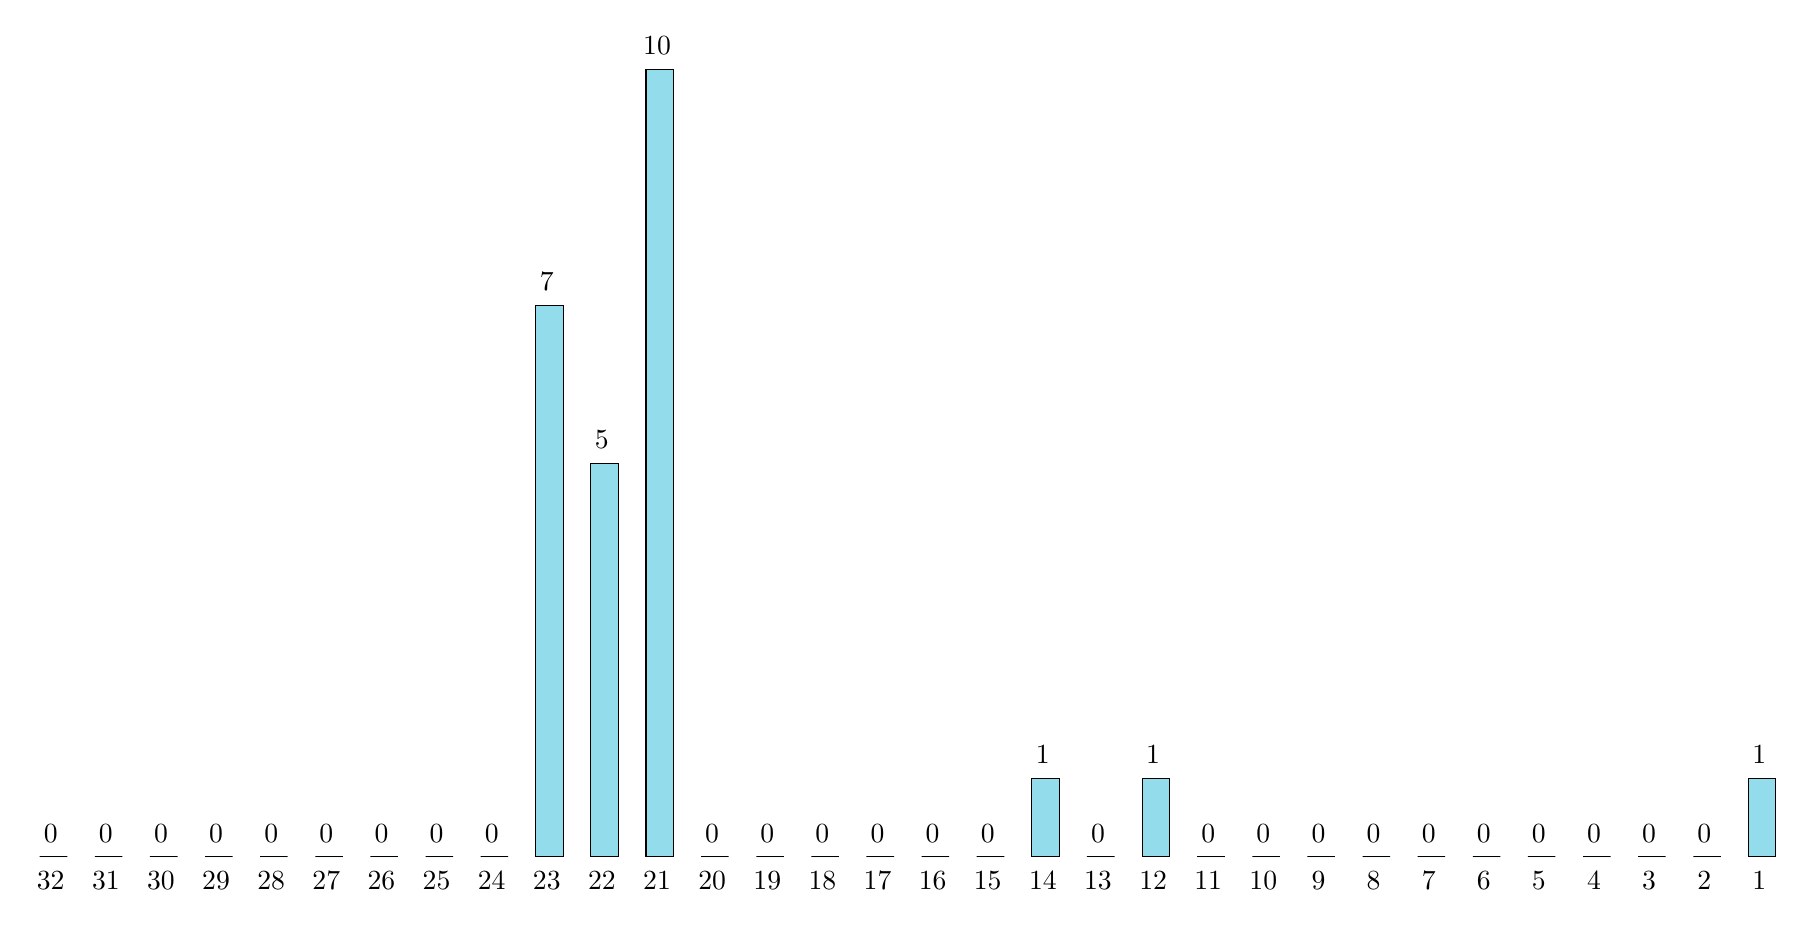
\begin{tikzpicture}[xscale=0.7,yscale=0.1]
	\draw[fill=niceblue] (0,0) rectangle (0.5+0,0.00) node at (0.2+0,3) {0};
	\draw[fill=niceblue] (1,0) rectangle (0.5+1,0.00) node at (0.2+1,3) {0};
	\draw[fill=niceblue] (2,0) rectangle (0.5+2,0.00) node at (0.2+2,3) {0};
	\draw[fill=niceblue] (3,0) rectangle (0.5+3,0.00) node at (0.2+3,3) {0};
	\draw[fill=niceblue] (4,0) rectangle (0.5+4,0.00) node at (0.2+4,3) {0};
	\draw[fill=niceblue] (5,0) rectangle (0.5+5,0.00) node at (0.2+5,3) {0};
	\draw[fill=niceblue] (6,0) rectangle (0.5+6,0.00) node at (0.2+6,3) {0};
	\draw[fill=niceblue] (7,0) rectangle (0.5+7,0.00) node at (0.2+7,3) {0};
	\draw[fill=niceblue] (8,0) rectangle (0.5+8,0.00) node at (0.2+8,3) {0};
	\draw[fill=niceblue] (9,0) rectangle (0.5+9,70.00) node at (0.2+9,73) {7};
	\draw[fill=niceblue] (10,0) rectangle (0.5+10,50.00) node at (0.2+10,53) {5};
	\draw[fill=niceblue] (11,0) rectangle (0.5+11,100.00) node at (0.2+11,103) {10};
	\draw[fill=niceblue] (12,0) rectangle (0.5+12,0.00) node at (0.2+12,3) {0};
	\draw[fill=niceblue] (13,0) rectangle (0.5+13,0.00) node at (0.2+13,3) {0};
	\draw[fill=niceblue] (14,0) rectangle (0.5+14,0.00) node at (0.2+14,3) {0};
	\draw[fill=niceblue] (15,0) rectangle (0.5+15,0.00) node at (0.2+15,3) {0};
	\draw[fill=niceblue] (16,0) rectangle (0.5+16,0.00) node at (0.2+16,3) {0};
	\draw[fill=niceblue] (17,0) rectangle (0.5+17,0.00) node at (0.2+17,3) {0};
	\draw[fill=niceblue] (18,0) rectangle (0.5+18,10.00) node at (0.2+18,13) {1};
	\draw[fill=niceblue] (19,0) rectangle (0.5+19,0.00) node at (0.2+19,3) {0};
	\draw[fill=niceblue] (20,0) rectangle (0.5+20,10.00) node at (0.2+20,13) {1};
	\draw[fill=niceblue] (21,0) rectangle (0.5+21,0.00) node at (0.2+21,3) {0};
	\draw[fill=niceblue] (22,0) rectangle (0.5+22,0.00) node at (0.2+22,3) {0};
	\draw[fill=niceblue] (23,0) rectangle (0.5+23,0.00) node at (0.2+23,3) {0};
	\draw[fill=niceblue] (24,0) rectangle (0.5+24,0.00) node at (0.2+24,3) {0};
	\draw[fill=niceblue] (25,0) rectangle (0.5+25,0.00) node at (0.2+25,3) {0};
	\draw[fill=niceblue] (26,0) rectangle (0.5+26,0.00) node at (0.2+26,3) {0};
	\draw[fill=niceblue] (27,0) rectangle (0.5+27,0.00) node at (0.2+27,3) {0};
	\draw[fill=niceblue] (28,0) rectangle (0.5+28,0.00) node at (0.2+28,3) {0};
	\draw[fill=niceblue] (29,0) rectangle (0.5+29,0.00) node at (0.2+29,3) {0};
	\draw[fill=niceblue] (30,0) rectangle (0.5+30,0.00) node at (0.2+30,3) {0};
	\draw[fill=niceblue] (31,0) rectangle (0.5+31,10.00) node at (0.2+31,13) {1};
	\draw (0.2+0,-3) node {32};
	\draw (0.2+1,-3) node {31};
	\draw (0.2+2,-3) node {30};
	\draw (0.2+3,-3) node {29};
	\draw (0.2+4,-3) node {28};
	\draw (0.2+5,-3) node {27};
	\draw (0.2+6,-3) node {26};
	\draw (0.2+7,-3) node {25};
	\draw (0.2+8,-3) node {24};
	\draw (0.2+9,-3) node {23};
	\draw (0.2+10,-3) node {22};
	\draw (0.2+11,-3) node {21};
	\draw (0.2+12,-3) node {20};
	\draw (0.2+13,-3) node {19};
	\draw (0.2+14,-3) node {18};
	\draw (0.2+15,-3) node {17};
	\draw (0.2+16,-3) node {16};
	\draw (0.2+17,-3) node {15};
	\draw (0.2+18,-3) node {14};
	\draw (0.2+19,-3) node {13};
	\draw (0.2+20,-3) node {12};
	\draw (0.2+21,-3) node {11};
	\draw (0.2+22,-3) node {10};
	\draw (0.2+23,-3) node {9};
	\draw (0.2+24,-3) node {8};
	\draw (0.2+25,-3) node {7};
	\draw (0.2+26,-3) node {6};
	\draw (0.2+27,-3) node {5};
	\draw (0.2+28,-3) node {4};
	\draw (0.2+29,-3) node {3};
	\draw (0.2+30,-3) node {2};
	\draw (0.2+31,-3) node {1};
	\end{tikzpicture}%
\end{landscape}

\section*{Produktivste Tageszeit?}%
\pdfbookmark[3]{Produktivste Tageszeit?}{hour_of_day}
\includegraphics[width=14cm]{stats/hour_of_day-crop}%

\section*{Produktivster Wochentag?}
\pdfbookmark[3]{Produktivster Wochentag?}{day_of_week}
\includegraphics[width=14cm]{stats/day_of_week-crop}%

\section*{Produktivster Monat?}%
\pdfbookmark[3]{Produktivster Monat?}{month_of_year}
\includegraphics[width=14cm]{stats/month_of_year-crop}%

\section*{Quellcode Zeilen?}%
\pdfbookmark[3]{Quellcode Zeilen?}{lines_of_code}
\includegraphics[width=14cm]{stats/lines_of_code-crop}%

\section*{Dateitypen?}%
\pdfbookmark[3]{Dateitypen?}{dateitypen}
\begin{center}%
	\begin{tabular}{lrD{.}{,}{1}rD{.}{,}{1}r}
	\textbf{Dateiendung} & \multicolumn{2}{c}{\textbf{Dateien}} & \multicolumn{2}{c}{\textbf{Zeilen}} & \textbf{Zeilen/Dateien} \\
	 & Anzahl & \% & Anzahl & \% & \\
	 & 5 & 22.73 & 47 & 3.01 & 9 \\
	tex & 16 & 72.73 & 1515 & 96.93 & 94 \\
\end{tabular}%
\end{center}%

\end{document}
